\chapter{Preliminaries}
\label{ch:preliminaries}

%------------------------------------------------
\section{What is Deep Learning for Software Engineering (\textit{DL4SE})?}

%------------------------------------------------
\section{Causal Inference Notation for Software Engineering}
\label{sec:pre-ci4se}
The ultimate goal of interpretability in Deep Learning for Software Engineering (\textit{DL4SE}) is to generate explanations of Neural Code Models' decisions represented as prediction performance (\ie Cross-Entropy or Next Token Prediction). A method to generate these explanations is based on the idea of estimating the effect of \textbf{\textit{interventions}} on the inputs or parameters that configure \nlms. When we collect datasets on possible cases that affect the generative process of \nlms, we are in fact searching for statistical or software properties that we can intervene upon to explain prediction performance. 

\begin{exmp}
\label{exmp:association}
Consider a simple Bayesian network to explain the performance of a given \nlm, an arrow that links buggy input code to model performance $Buggy\to Perf$. The variables $Buggy$ and $Perf$ are dependent, both variables embody a \textit{program repair intervention}. Therefore, if we want to define the joint distribution $p(Buggy,Perf)$ to represent the network, we must specify by Bayes' rule using the prior $p(Buggy)$ and the conditional probability $p(Perf|Buggy)$. Nonetheless, such a joint distribution can be computed as well in the opposite direction  $Perf\to Buggy$ using the same Bayes' rule for a prior $p(Perf)$ and conditional $p(Buggy|Perf)$. The fact that the joint distribution can be represented with both networks is non-intuitive since we know from experience and software understanding that the model performance cannot give rise to a bug in the original input. In other words, the relationship between these variables is asymmetric or \textit{causal}. Hence, we expect that buggy snippets affect the performance of \nlms, not the other way around.
\end{exmp}

A first attempt to address the relationship in Ex.~\ref{exmp:association} would be computing a correlation coefficient $\rho_{TY}\approx p(Y|T)=p(Perf|Buggy)$, where $T$ is a binary \textit{treatment} that represents the \textit{debugging} process and $Y$ is a \textit{potential outcome} that corresponds to the model performance. This coefficient, however, is still symmetric: if $T$ is correlated with $Y$, then $Y$ is equally correlated with $T$. \textit{Causal networks} allow us to model causal asymmetries where directionality goes beyond probabilistic dependence. These causal models represent the mechanism by which data \textit{were generated} \cite{Pearl2016Causality}. Instead of testing whether $Buggy$ and $Perf$ are conditionally dependent, \textit{causation} asks which variable \textit{responds} to the other one: $Buggy$ to $Perf$ or $Perf$ to $Buggy$? \cite{Pearl2016Causality}.

\marginnote{
\begin{definition}
\label{def:causation}
  \textbf{Causation.} A variable $T$ is a \textit{cause} of $Y$ if the variable $Y$ depends on $T$ to determine its value. Formally, the value of $Y$ was \textit{assigned} on the basis of what it is known about $T$. In other words, the value of $Y$ is determined by a \textit{\textbf{structural equation}} $Y=f_y(T,U_y)$ and the arrow $T\to Y$. The $U$ variables in these equations represent \textit{unmodeled} variables that are exogenous to the causal network but disturb the functional relationship between the outcome and its treatment \citep{Scholkopf2022}.    
\end{definition}
}

Similarly, we can define a structural function for the treatment $T=f_t(U_t)$ that depends only on $U$ disturbances assuming that no \textit{common causes} exists between outcomes and treatments. A common cause is a random variable $Z$ that causally influence two variables that are initially perceived as statically dependant ($T \not\!\perp\!\!\!\perp Y$). However, this dependency can be explained by the underlying influence of $Z$ on the effects, making the effects in fact conditionally independent ($T \perp\!\!\!\perp Y | Z$). Therefore, there exist more complex causal relationships between treatments and outcomes that we are able to model with structural equations that corresponds to a \textit{\textbf{Structural Causal Model}} (SCM). 

\marginnote{
\begin{definition}
\label{def:scm}
  \textbf{Structural Causal Models.} These directed acyclic graphs (DAGs) describe direct parent-child relationships, instead of probabilistic dependencies, among random variables $X_i$. The value $x_i$ of each variable $X_i$ is defined by the structural equations $x_i = f_i(PA_i,U_i)$ where $PA_i = {X_j: X_j \to X_i}$ denotes the set of parents or direct causes of $X_i$. This model allow us to introduce a graphical definition of causation  \citep{Scholkopf2022,Pearl2009Causality}.
\end{definition}
}

SCMs are stable mechanisms that remain invariant to local changes unlike probabilities computed by Bayesian networks \citep{Pearl2016Causality}. This peculiar characteristic is responsible for enabling us to estimate quantitatively the results of an action or intervention in the graph without actually performing it in controlled settings (\ie randomized experiments). In other words, SCMs provide a framework for \textit{counterfactual reasoning}. The mathematical tool employed to perform these interventions is the $do(\cdot)-operator$ \citep{Pearl2009Causality}. For instance, if we want to estimate how fixed code affects the performance of a \nlm, we just need to compute the action $p(Perf|do(Buggy=False))$ (Eq.~\ref{eqn:do-1}). These type of actions are \textit{interventional} distributions since we \textbf{set} the value of $Buggy$ to $False$. Note that this interventional distribution is not necessarily $p(Perf|Buggy=False)$ (Eq.~\ref{eqn:do-2}). This latter distribution is \textit{observational} since we are \textit{conditioning} the performance on the value of the $Buggy$ variable. Intervening on a variable in a SCM means fixing its value and, therefore, changing the value of other variables of the network as a result. Conversely, conditioning on a variable means narrowing the cases that the outcome takes once we assign a value to the treatment.   

\begin{figure}[h]
		\centering
		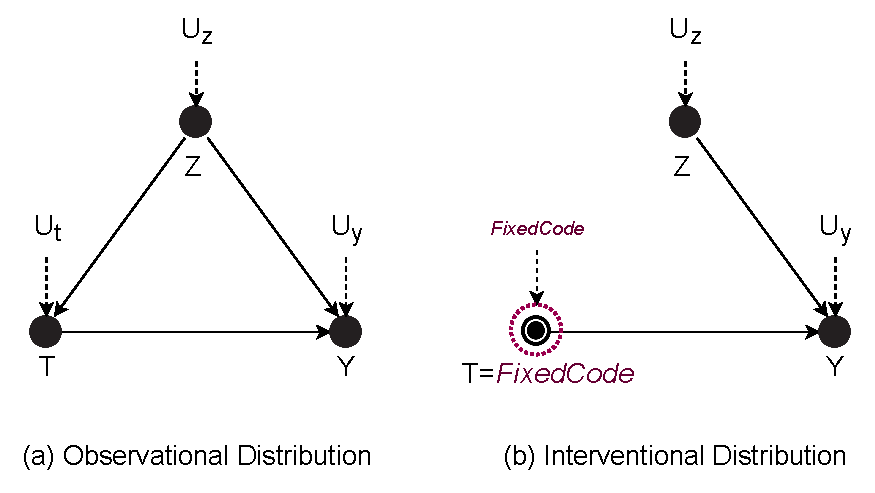
\includegraphics[width=0.9\textwidth]{graphics/preliminaries/fig_1_causalnet.pdf}
		\caption{(a) \textit{Structural Causal Model} representing cause-effect relationships of program repair in \nlms. (b) The \textit{SCM} after intervening the treatment with \textit{Fixed Code}.}
        \label{fig:scm}
\end{figure}

\begin{exmp} 
\label{exmp:scm}
Consider Fig.~\ref{fig:scm} a generalization of the buggy influence on a deep model's performance. The first graph is a SCM composed of a treatment variable $T=Buggy$ and potential outcome $Y=Perf$. In addition, we identified some common causes $Z=SE_{Metrics}$ for treatments and potential outcomes. These common causes (or covariates) are Software Engineering quality metrics (\eg Lines of Code, McCabe Complexity, Size of Methods). Now we want to perform the intervention $do(Buggy=False)$ which is the same as $do(T=FixedCode)$. The second graph depicts this program repair intervention. Note that fixing the value of $T$ makes the SCM change by eliminating the effect or influence arrow of the common cause $Z$ to the treatment. The disturbance $U_t$ is also eliminated. This elimination process of input arrows to fixed variables is formally known as \textit{graph surgery}. Both $do(\cdot)-operator$ and graph surgery allow us to untangle causal relationships from mere correlations \citep{Pearl2009Causality}. The law of total probabilities and invariance principle are required to compute the observational and interventional distributions \citep{Scholkopf2022}:
\end{exmp}

\begin{subequations}
\begin{align}
p(Y|do(t=FixedCode)) &=\sum_{z \in _{metrics}}p(Y|z,t)p(t)\label{eqn:do-1} \\
p(Y|t=FixedCode) &= \sum_{z \in _{metrics}}p(Y|z,t)p(t|z) \label{eqn:do-2} 
\end{align}
\label{eqn:do-all-lines}
\end{subequations}

Note that Eq.~\ref{eqn:do-1} differs from  Eq.~\ref{eqn:do-2}: the prior $p(t)$ in contrast to $p(t|z)$, which is precisely the link that is eliminated in the SCM. Eq.~\ref{eqn:do-1} is formally known as the \textbf{\textit{adjustment formula}}. This formula is one of the building blocks in causal inference since it helps us to adjust common causes or control for covariates to compute the \textit{treatment or causal effect} \citep{Pearl2009Causality,Pearl2016Causality}.

\marginnote{
    \begin{definition}\label{def:effect}
    \textbf{Treatment Effects.} Given a Structural Causal Graph where a set of variables $PA$ denotes the parents of $T$, the treatment effect of T on Y is given by $p(Y=y|do(T=t))$ in Eq.~\ref{eq:effect}
    \end{definition}
}

\david{contextualize function below}
\begin{subequations}
    {%\tiny
        \begin{align}
        &p(Y=y|do(T=t)) &&=  \label{eq:effect-1}\\
        &\Sigma_z p(Y=y|T=t,PA=z)p(PA=z)  &&= \label{eq:effect-2}\\
        &\Sigma_z p(T=t,Y=y,PA=z)/p(T=t|PA=z) \label{eq:effect-3}
        \end{align}
    }
\label{eq:effect}
\end{subequations}

In our initial causal statement, we generally accept that buggy code \textit{causes} a \nlm to perform poorly. Although the causal statement is true, it is not guaranteed that every buggy snippet is certain to make a model perform poorly. Therefore, causal relationships are \textbf{uncertain}. This uncertainty is captured by employing conditional probabilities described in Eq.~\ref{eq:effect-1}. In order to compute treatment effects, we need to connect observational data with our interventional distribution. Note Eq.~\ref{eq:effect-3} is obtained with Bayes' rule and algebraic manipulation once we multiply and divide by the term $p(T=t|PA=z)$. This term is a conditional probability known as the \textit{propensity score}. This propensity score and the join probability of all the nodes are distributions that can be obtained from data \citep{Pearl2016Causality}. We explain this connection for code generation in Sec. \S~\ref{sec:appII-approach}. 

\david{Re-write the following paragraph to generalize the thesis document.}
In summary, our interpretability methodology \codegen is based on the idea of proposing causal queries given a SCM. These causal queries are obtained by estimating an interventional distribution where the potential outcome is generally a prediction performance value of Neural Code Model under study and the treatments are a set of software-based properties that help us construct explanations about the generative model.

%------------------------------------------------
\subsection{Code Traceability}

%------------------------------------------------
\subsection{Code Generation}